\section{Event preselection}

Events used in the $t\bar{t}H$ search share part of the preselection described in section \ref{sec:vlq:presel}. Events are required to pass the same ``event cleaning'' and to  satisfy the single-lepton requirements, both at the trigger and offline-selection levels. Events are further required to have at least four jets\footnote{In the following, the term ``jet'' is used to refer to a small-$R$ jet since no large-$R$ jets are used in this search.} and at least two $b$-tagged jets ($70\%$ operating point). 
No selection is applied on the $\MET$ and the $W$-boson transverse mass; the signal-to-background ratio of the analysis is not altered by the relaxation of the selection since $t\bar{t}H$ and the main background ($t\bar{t}$) are affected in the same way. Nevertheless, it brings an increase in signal acceptance that helps to improve the statistical precision of the analysis.
Table \ref{tab:tth:presel} summarises the requirements described above and referred to as the ``preselection''. 


\begin{table}[h!b]\footnotesize
\begin{center}
\begin{tabular}{c|c|c}
  \hline \hline
  \multicolumn{3}{c}{Preselection requirements}\\
  \hline
   Requirement & $t\bar{t}H$ search & $T\bar{T}$/$t\bar{t}t\bar{t}$ search \\
  \hline
  Event cleaning & \checkmark & \checkmark\\
  Trigger & Single-lepton trigger &Single-lepton trigger\\
  Leptons & =1 isolated e or $\mu$ & =1 isolated e or $\mu$ \\
  Jets & $\ge$4 jets & $\ge$5 jets\\
  $b$-tagging & $\ge$2 $b$-tagged jets $@70\%$ OP &$\ge$2 $b$-tagged jets $@77\%$ OP\\
  \MET & - & \MET > 20 GeV \\
  Other \MET-related & - &\MET + $m_{T}^{W}$ > 60 GeV\\  
 \hline \hline
\end{tabular}
\captionsetup{width=0.85\textwidth}  \caption{\small Summary of preselection requirements for the $t\bar{t}H$ search. For comparison, a summary of preselection requirements made in the 1-lepton channel for the search described in section \ref{sec:vlq:presel} is reported as well. Here $m_{\rm T}^{W}$ is the transverse mass of the lepton and the \MET vector. }
\label{tab:tth:presel}
\end{center}
\end{table}

\subsection{Comparison between data and prediction}

Figure \ref{sec:tth:fig:1ldatamc}  presents basic kinematic variables at preselection level, showing reasonable agreement between data and the background prediction. As indicated for the search described in chapter \ref{chp:VLQ}, in this case the observed discrepancies are covered by systematic uncertainties, shown by the hashed area. Differences in the systematic uncertainties treatment compared to that discussed in section \ref{chp:vlq:sec:syst} are summarised in section \ref{sec:tth:systunc}.


\begin{figure}[p]
\begin{subfigure}{0.33\textwidth}
  \centering
  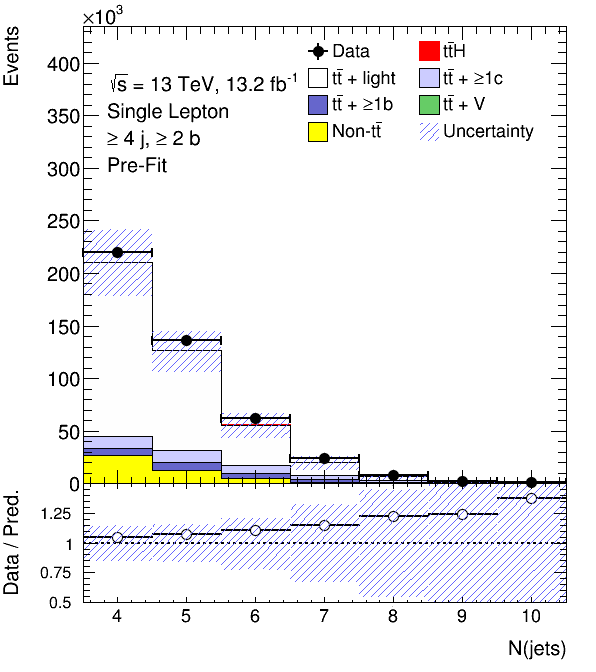
\includegraphics[width=0.9\textwidth]{figures/ttH/presel/ljets_nJets_ge4jge2b.png}
  \caption{}
  \label{}
\end{subfigure}
\begin{subfigure}{0.33\textwidth}
  \centering
  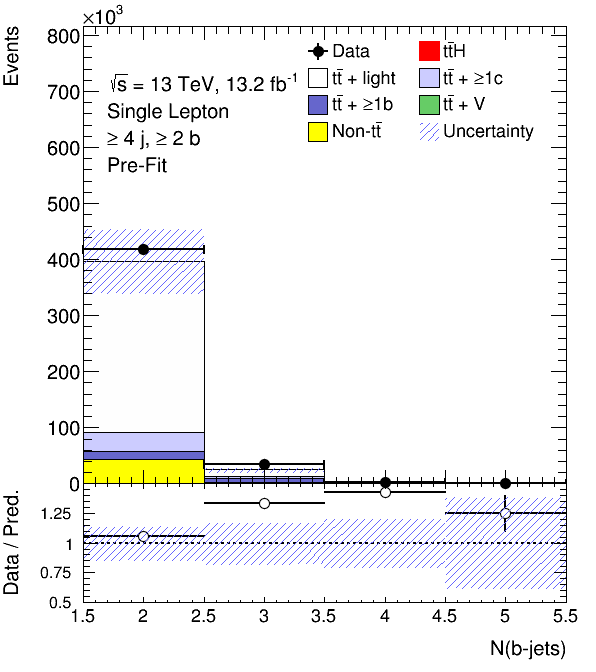
\includegraphics[width=0.9\textwidth]{figures/ttH/presel/ljets_nBJets_ge4jge2b.png}
  \caption{}
  \label{}
\end{subfigure}
\begin{subfigure}{0.33\textwidth}
  \centering
  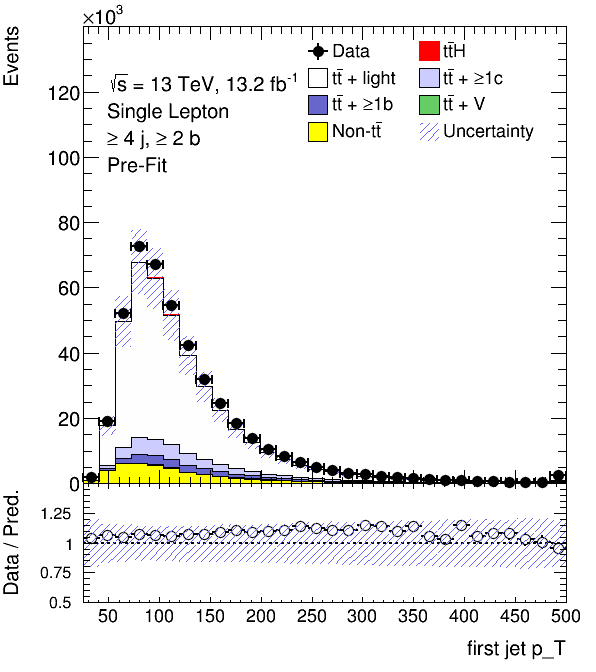
\includegraphics[width=0.9\textwidth]{figures/ttH/presel/ljets_jet1Pt_ge4jge2b.png}
  \caption{}
  \label{}
\end{subfigure}
\begin{subfigure}{0.33\textwidth}
  \centering
  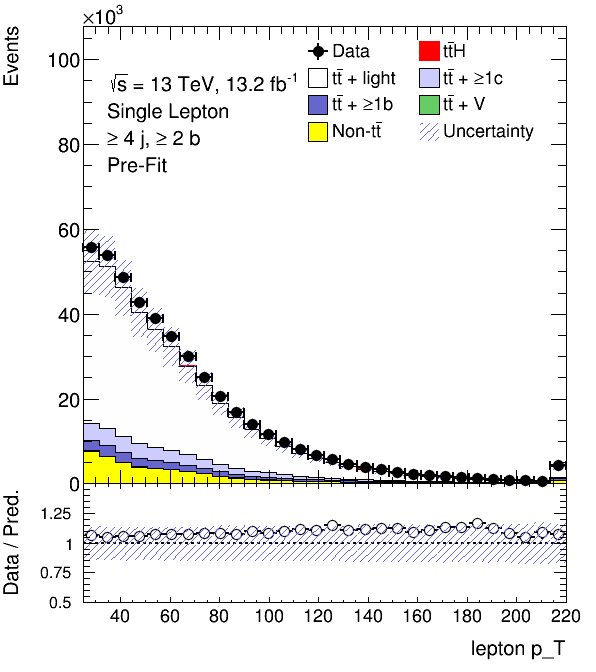
\includegraphics[width=0.9\textwidth]{figures/ttH/presel/ljets_leptonPt_ge4jge2b.png}
  \caption{}
  \label{}
\end{subfigure}
\begin{subfigure}{0.33\textwidth}
  \centering
  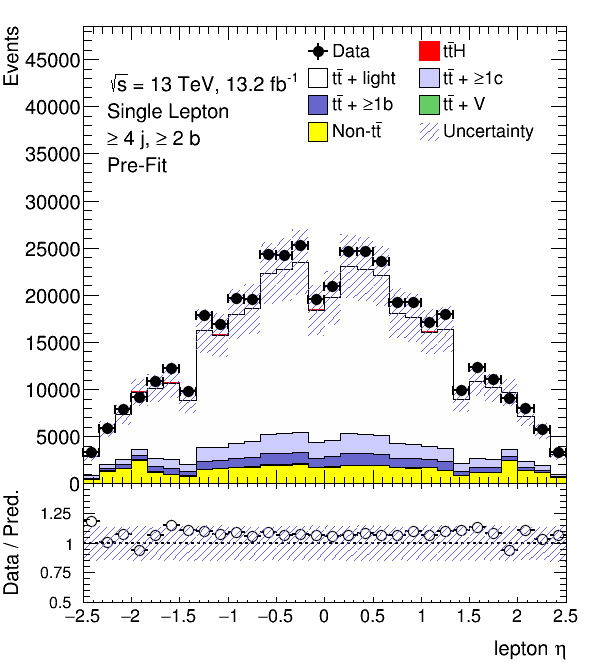
\includegraphics[width=0.9\textwidth]{figures/ttH/presel/ljets_leptonEta_ge4jge2b.png}
  \caption{}
  \label{}
\end{subfigure}
\begin{subfigure}{0.33\textwidth}
  \centering
  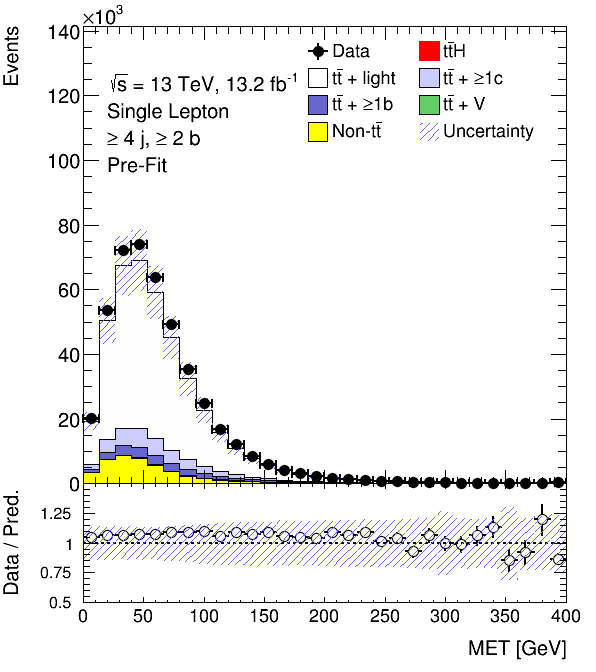
\includegraphics[width=0.9\textwidth]{figures/ttH/presel/ljets_MET_ge4jge2b.png}
  \caption{}
  \label{}
\end{subfigure}
\begin{center}
\begin{subfigure}{0.33\textwidth}
  \centering
  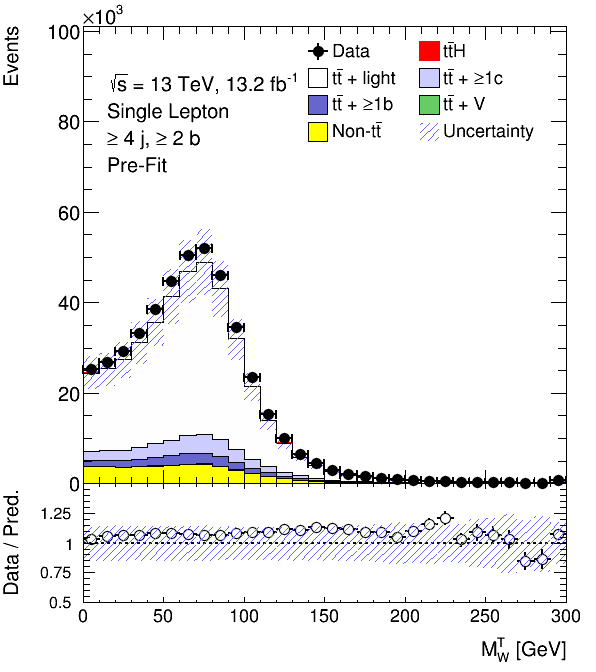
\includegraphics[width=0.9\textwidth]{figures/ttH/presel/ljets_MTW_ge4jge2b.png}
  \caption{}
  \label{}
\end{subfigure}
\begin{subfigure}{0.33\textwidth}
  \centering
  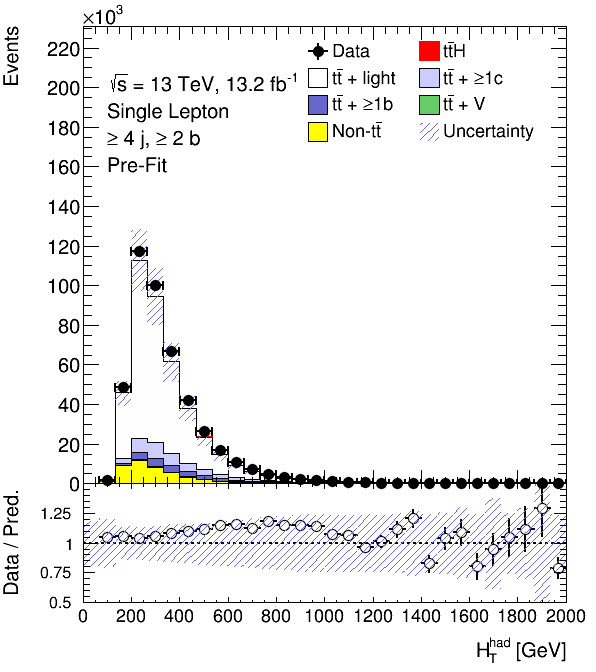
\includegraphics[width=0.9\textwidth]{figures/ttH/presel/ljets_HThad_ge4jge2b.png}
  \caption{}
  \label{}
\end{subfigure}
\end{center}
\captionsetup{width=0.85\textwidth}  \caption{\small Comparison between data and prediction in at the preselection level in the $t\bar{t}H$ search for (a) jet multiplicity, (b) $b$-tag multiplicity, (c) leading jet $\pt$, (d) lepton $\pt$, (e) lepton $\eta$, (f) \MET , (g) transwerse mass of the W boson ($m_{\rm T}^{W}$), and (h) scalar sum of jet $\pt$ ($H_{T}^{\rm had}$). The hashed area represents the total uncertainty on the background.}
\label{sec:tth:fig:1ldatamc}
\end{figure}